\bframe{}
    \fig{i/mills.pdf}{Mills et al}{fig:rbc1}
\eframe

\bframe{Big and small diameters}
    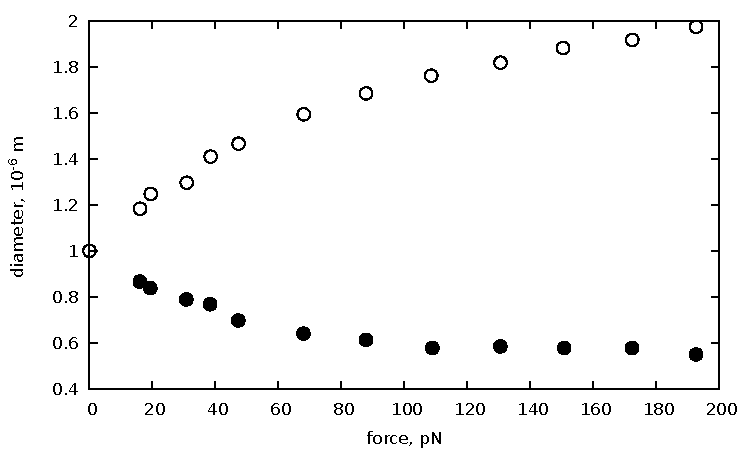
\includegraphics[width=\textwidth]{gp/str.pdf}
\eframe

\bframe{Number of ``pulled beads'' dependence}
    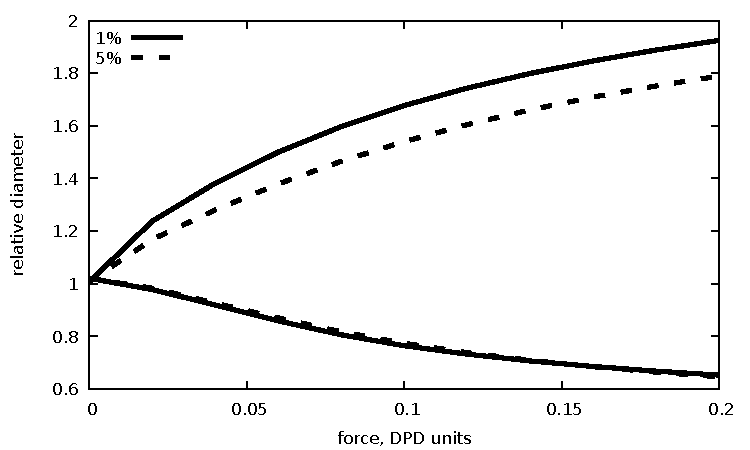
\includegraphics[width=\textwidth]{gp/bead.pdf}
\eframe

\bframe{Number of ``pulled beads'' dependence}
    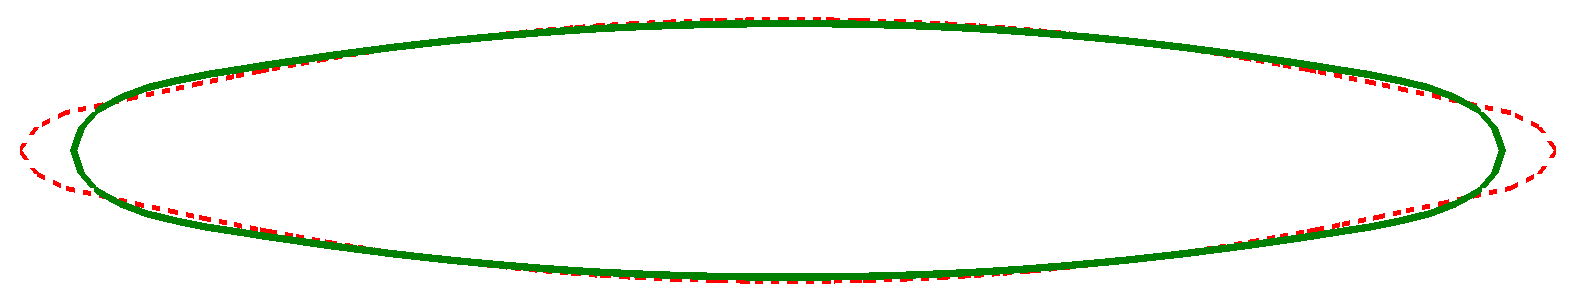
\includegraphics[width=\textwidth]{visit/v.png}
\eframe

\bframe{Equilibrium shape}
\bcc  
  \bc
     \fig{i/A0_crossY.png}{}{}
  \ec
  \bc
     \fig{i/A0_crossZ.png}{}{}
  \ec
\ecc  
\eframe

\bframe{Equilibrium shape}
    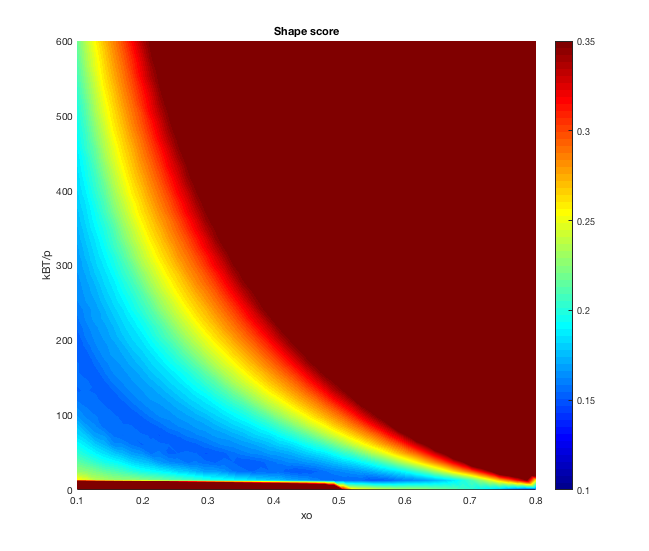
\includegraphics[width=0.9\textwidth]{i/score.png}
\eframe

\bframe{Stretched shape}
\bcc  
  \bc
     \fig{i/A500_crossX.png}{}{}
  \ec
  \bc
     \fig{i/A500_crossZ.png}{}{}
  \ec
\ecc  
\eframe

\bframe{Best fit}
    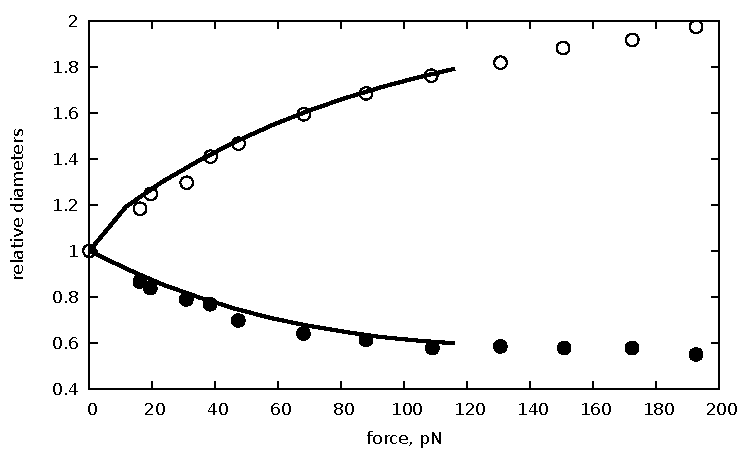
\includegraphics[width=\textwidth]{gp/best.pdf}
\eframe

\bframe{Sucking cap?}
\bcc  
  \bc
     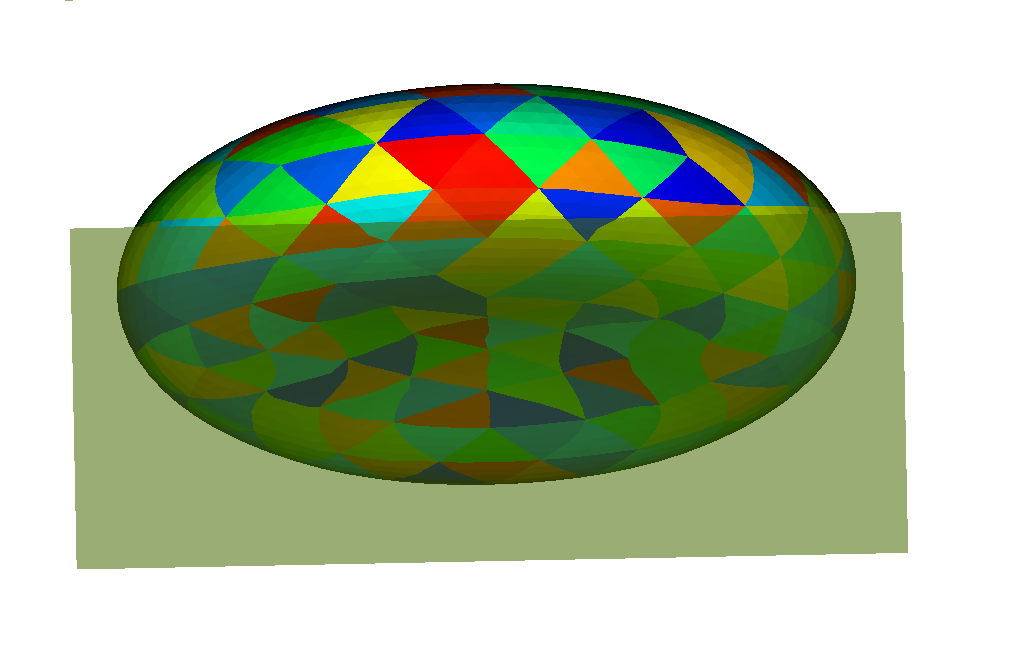
\includegraphics[width=1.2\textwidth]{i/glass0.png}
  \ec
  \bc
     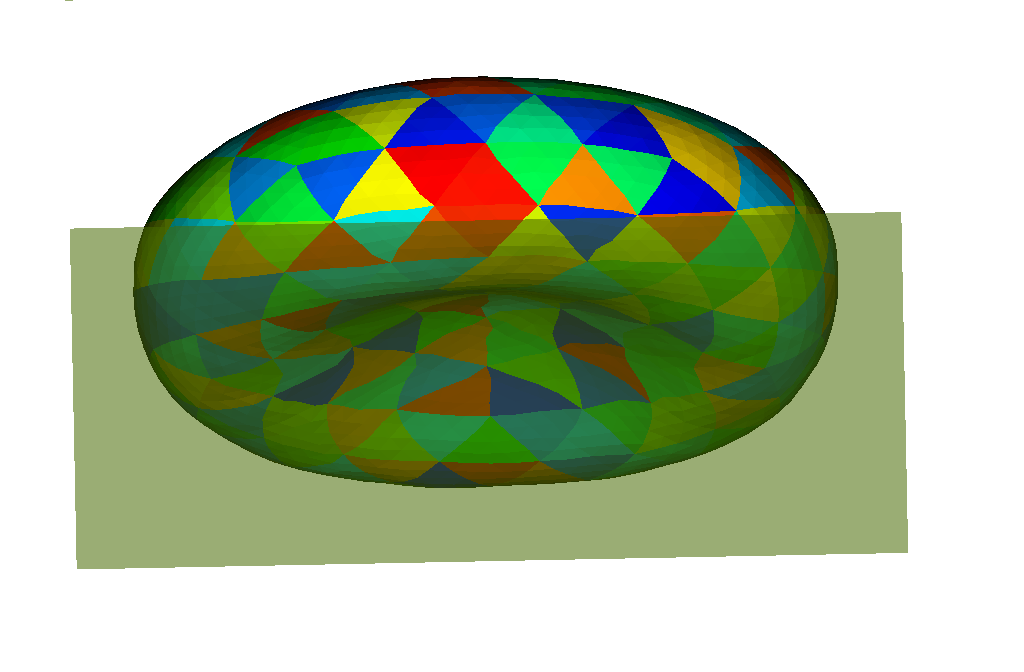
\includegraphics[width=1.2\textwidth]{i/glass1.png}
  \ec
\ecc  
\eframe

\bframe{Sucking cap?}
     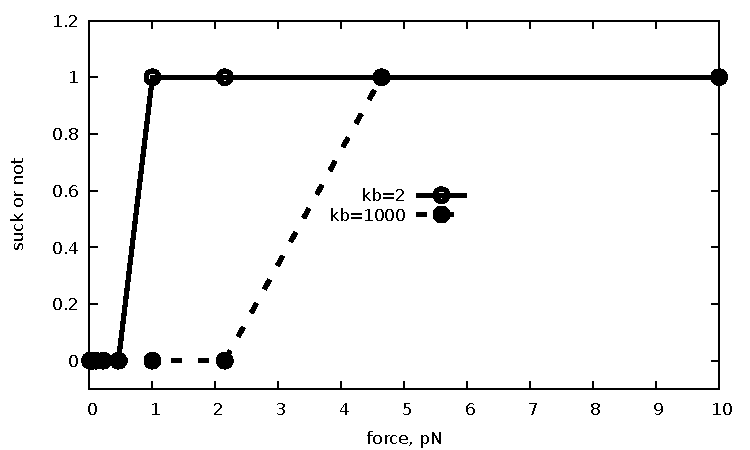
\includegraphics[width=\textwidth]{gp/suck.pdf}
\eframe
